% \documentclass[a4paper,10pt]{article}
% \usepackage[utf8x]{inputenc}
% 
% 
% %opening
% \title{Exploring Your Favorite Corpus with The Topic Browser}
% \author{}
% 
% \begin{document}
% 
% \maketitle
% 

% % 
% % \section{Why?}

% % 
% % Previous visualization attempts....
% % 
% % Why they fail
% % 
% % 
% % 
% % 
% % 
% % \subsection{...but their output is hard for humans to digest}
% % \subsection{Topics aren't isolated entities, but form a network in combination
% % with documents, words, authors, etc.}
% % \subsection{This network is implied by a topic model, but generally not made
% % explicit (?)}
% % \subsection{More informative}
% % Experience suggests that an explicit representation of the relationships between
% % all entities modeled and makes topic model output more informative and usable.
% % [We're in the process of formally validating this claim.]
% % 

% 
% 
% 
% 
% 
% \end{document}

%
% File acl-hlt2011.tex
%
% Contact: gdzhou@suda.edu.cn
%%
%% Based on the style files for ACL2008 by Joakim Nivre and Noah Smith
%% and that of ACL2010 by Jing-Shin Chang and Philipp Koehn


\documentclass[11pt]{article}
\usepackage{acl-hlt2011}
\usepackage{times}
\usepackage{latexsym}
\usepackage{amsmath}
\usepackage{multirow}
\usepackage{url}
\usepackage{graphicx}
\DeclareMathOperator*{\argmax}{arg\,max}
\setlength\titlebox{6.5cm}    % Expanding the titlebox

\title{Exploring Your Favorite Corpus with The Topic Browser}
\author{Matthew J. Gardner, Joshua Lutes, Josh Hansen, Jeff Lund, Dan Walker, Eric Ringger, \and Kevin Seppi\\
Department of Computer Science\\
Brigham Young University\\
\tt \{mjg82,jlutes,joshhansen\}@byu.edu, \{jefflund,danwalkeriv\}@gmail.com\\
\tt \{ringger,kseppi\}@cs.byu.edu}

\date{}

\begin{document}
\maketitle

% \begin{abstract}
% Problem: You're developing yet another LDA variant and want to get a feel for its output.
% Solution: Use the Topic Browser to check things out at the topic, word, and document levels.
% Problem: You have a mountain of documents so vast that no non-cyborg could read them all.
% Solution: Get the Topic Browser and do some interactive, topic-based exploration.
% Problem: The public has difficulty accessing the treasure trove of documents your institution wishes to make available.
% Solution: Expose it to the world via the Topic Browser's web interface.
% \end{abstract}

\begin{abstract}
The Topic Browser is an open-source\footnote{Licensed under the terms of the
Affero General Public License, version 3.}  web application for interactive
exploration and visualization of topics and documents. Mallet LDA output is used
as input. We explain why such a tool is warranted, what it is capable of, and
how to use it to explore the corpus (or topic model) of your choice.
\end{abstract}

\section{Introduction}
Since their introduction in 2003, LDA-based topic models have been extended to
account for time, authors, citations, multiple languages, etc. [][][][][]
Baseline LDA generates a topic assignment per (non-stop) token -- a massive
output in the gigaword era. Humans are incapable of fully assimilating the
resulting models, calling for more effective means of characterizing and
visualizing the output.

The Topic Browser is an open-source web application for interactive exploration
and visualization of document collections. All entities implied by topic model output are first-class citizens in the Topic
Browser. 

% \subsection{Entities}
% \begin{figure}[ht]
%  \centering
%  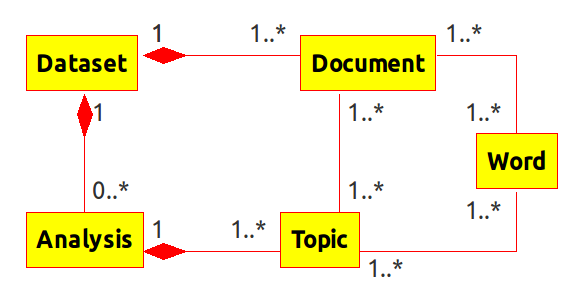
\includegraphics{topic_browser_object_model_transparent.png}
%  % topic browser object model transparent.png: 582x293 pixel, 96dpi, 15.40x7.75
% cm, bb=0 0 436 220
%  \caption{The Topic Browser object model}
%  \label{fig:object_model}
% \end{figure}

\subsection{Topics}

\subsection{Documents}

\subsection{Words}

\subsection{Metrics}
topic, topic-topic, document, document-document

\subsection{Charts}



\subsection{Topic ``Maps"}
With topic-to-topic relationships described by means of pairwise topic metrics,
graph-based visualization of the topic space becomes straightforward. In our
current implementation, we construct a topic graph G = (N, E) as follows:
\begin{itemize}
\item $N$ is a set of $|T|$ nodes such that $\forall_{t\in T} weight(N_{t}) =
\tau(t)$ where $\tau$ is a topic metric.
\item $E$ is a set of $|T|^2$ edges such that $\forall_{t\in T}\forall_{u\in T}
weight(E_{t,u}) = \mu(t,u)$ where $\mu$ is a pairwise topic metric.
\end{itemize}

We use the Gephi Toolkit\footnote{http://www.gephi.org} to generate such graphs
and render them as images.
\begin{figure}
  \begin{center}
  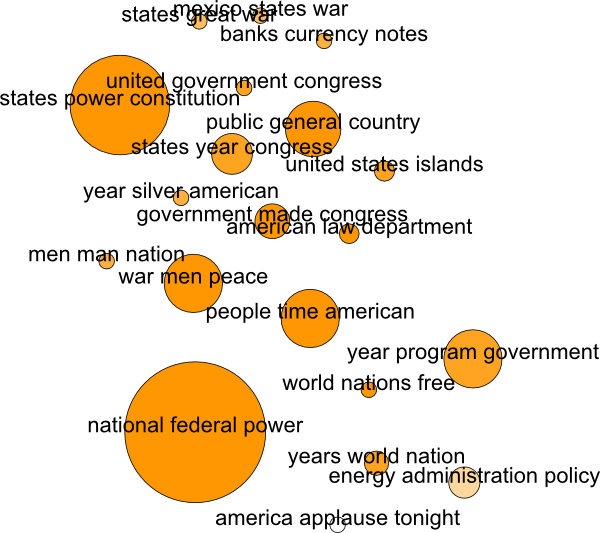
\includegraphics[width=200px,keepaspectratio=true]{./topic_map_example.png}
  \caption{}
  \end{center}
\end{figure}
% \begin{center}
%  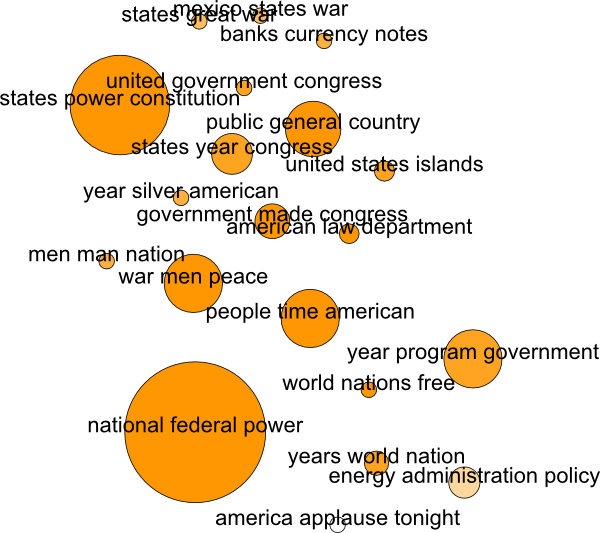
\includegraphics[width=200px,keepaspectratio=true]{./topic_map_example.png}
%  % topic_map_example.png: 600x533 pixel, 57dpi, 26.76x23.77 cm, bb=0 0 759 674
% \end{center}

\subsection{Topic Name Schemes}
As LDA does not assign names to the topics it generates, automatic generation of
topic names is of interest to researchers wishing to make topic models
human-usable. Research in this area is ongoing (CITATION???). In order to
facilitate investigations in this area, we equipped the Topic Browser with a
fully pluggable topic naming system. Any number of topic name schemes can be
used to produce names for all topics in an analysis. Within the user interface
users can select a name scheme, which is then reflected throughout the
interface. By default we use ''Top2`` (the name is a concatenation of the two
words with the highest $P(w|z)$ for a given topic $z$), but any number of
alternative schemes can be imagined and implemented. (MAYBE SHOW TF-ITF?)

\section{Data Import Backend}
SHOW DEPENDENCY GRAPH?
Automatically turning a raw document collection into an interactive browsing
experience requires extensive preprocessing. Documents must be converted into a
representation accepted by the topic model learner. Topics must then be inferred
and model output indexed. Additionally, metrics must be computed, topic names
generated, and graphs rendered before they become accessible via the user
interface. Unsurprisingly, the dependencies in the import process form a DAG. To
improve the efficiency and usability of the data import pipeline we built a
command-line frontend based on the \verb/doit/ task automation tool, written in
Python.\footnote{http://doit.sourceforge.net/}

The main \verb/doit/ build script is \verb/dodo.py/. Some example invocations:
\begin{itemize}
 \item \verb/dodo.py/: Builds all targets
 \item \verb/dodo.py list/: Lists the available top-level tasks (sub-tasks are not displayed)
 \item \verb/dodo.py clean -c mallet/: Cleans the Mallet files
\end{itemize}

% Useful commands:
%  dodo.py list #Lists the available top-level tasks (sub-tasks are not displayed)
%  dodo.py #Builds everything!
%  dodo.py clean -c mallet #Cleans the mallet files
%  dodo.py metrics #Computes all metrics
%  dodo.py topic_metrics #Computes just the topic metrics
%  dodo.py topic_metrics:document_entropy #Computes just the document entropy topic metric
%  dodo.py clean topic_metrics:document_entropy #Cleans just the document entropy topic metric
%
%NOTE: probably necessary to do 'dodo.py forget' when switching between datasets/analyses.

how to set different datasets

\subsection{Adding Support For Your Dataset}
The \verb/build/ Python module contains dataset-specific import scripts.
Generally, a sub-module contains the scripts for a particular dataset. The
scripts for the default State of the Union Addresses dataset, for example,
reside in \verb/build.state_of_the_union/. The main build file for the dataset
is \verb#build/state_of_the_union/state_of_the_union.py#. This file is
referenced within the root \verb/dodo.py/ build script by setting the
\verb/build/ variable:
\begin{verbatim}
 build = "state_of_the_union/state_of_the_union"
\end{verbatim}

At a minimum, the dataset-specific build file should contain the following:
\begin{itemize}
 \item Declaration of \verb/dataset_name/ variable.
   \newline Example: \verb/dataset_name = "state_of_the_union"/.
 \item Declaration of \verb/dataset_description/ variable.
   \newline Example: \verb/dataset_description = "State of the Union Addresses
1790-2010"/.
 \item Definition of \verb/copy_and_transform_dataset/ \verb/doit/ task.
Example:
\begin{verbatim}
def task_copy_and_transform_dataset():
  task = dict()
  task['actions'] = [
    (extract_state_of_the_union,
    [dataset_dir+'/'+chron_list_filename,
     dataset_dir+'/'+addresses_filename,
     files_dir]
    )
  ]
  task['clean'] = [
    'rm -rf '+files_dir
  ]
  task['uptodate'] = [os.path.exists(files_dir)]
  return task
\end{verbatim}

\end{itemize}

% \section{Credits}
% 
% This document has been adapted from the instructions for earlier ACL proceedings, including those for ACL-2008 by Johanna D. Moore, Simone Teufel, James Allan, and Sadaoki Furui, those for ACL-2005 by Hwee Tou Ng and Kemal Oflazer, those for ACL-2002 by Eugene Charniak and Dekang Lin, and earlier ACL and EACL formats. Those versions were written by several people, including John Chen, Henry S. Thompson and Donald Walker. Additional elements were taken from the formatting instructions of the {\em International Joint Conference on Artificial Intelligence}.
% 
% \section{Introduction}
% 
% The following instructions are directed to authors of papers submitted to ACL-HLT-2011 or accepted for publication in its proceedings. All authors are required to adhere to these specifications. Authors are required to provide a Portable Document Format (PDF)
% % das: removed reference to PostScript
% % and PostScript
% version of their papers. \textbf{The proceedings will be printed on US-Letter paper}. Authors from countries in which access to word-processing systems is limited should contact the publication chair Guodong Zhou ({\tt gdzhou@suda.edu.cn}) as soon as possible.
% 
% 
% \section{General Instructions}
% 
% Manuscripts must be in two-column format. Exceptions to the two-column format include the title, authors' names and complete addresses, which must be centered at the top of the first page, and any full-width figures or tables (see the guidelines in Subsection~\ref{ssec:first}). {\bf Type single-spaced}. Start all pages directly under the top margin. See the guide-lines later regarding formatting the first page.
% 
% The maximum length of a manuscript is eight (8) pages for the main conference, printed single-sided, plus two (2) pages for references (see Section~\ref{sec:length} for additional information on the maximum number of pages).  Do not number the pages.
% 
% \subsection{Electronically-available resources}
% 
% ACL-HLT-2011 provides this description in \LaTeX2e (acl-hlt2011.tex) and PDF format (acl-hlt2011.pdf), along with the LATEX2e style file used to format it (acl-hlt2011.sty) and an ACL bibliography style (acl.bst). These files are all available at \url{http://www.acl2011.org}.  A Microsoft Word template file (acl-hlt2011.dot) is also available at the same URL. We strongly recommend the use of these style files, which have been appropriately tailored for the ACL-HLT-2011 proceedings. If you have an option, we recommend that you use the \LaTeX2e version. \textbf{If you will be using the Microsoft Word template, we suggest that you anonymize your source file so that the pdf produced does not retain your identity.} This can be done by removing any personal information from your source
% document properties.
% 
% 
% \subsection{Format of Electronic Manuscript}
% \label{sect:pdf}
% 
% For the production of the electronic manuscript you must use Adobe's
% Portable Document Format (PDF). This format can be generated from
% postscript files: on Linux/Unix systems, you can use {\tt ps2pdf} for this
% purpose; under Microsoft Windows, you can use Adobe's Distiller, or
% if you have {\tt cygwin} installed, you can use {\tt dvipdf} or
% {\tt ps2pdf}.  Note
% that some word processing programs generate PDF which may not include
% all the necessary fonts (esp. tree diagrams, symbols). When you print
% or create the PDF file, there is usually an option in your printer
% setup to include none, all or just non-standard fonts.  Please make
% sure that you select the option of including ALL the fonts.  {\em Before sending it, test your PDF by printing it from a computer different from the one where it was created}. Moreover,
% some word processor may generate very large postscript/PDF files,
% where each page is rendered as an image. Such images may reproduce
% poorly.  In this case, try alternative ways to obtain the postscript
% and/or PDF.  One way on some systems is to install a driver for a
% postscript printer, send your document to the printer specifying
% ``Output to a file'', then convert the file to PDF.
% 
% Additionally, it is of utmost importance to specify the {\bf US-Letter format} (8.5in $\times$ 11in) when formatting the paper. When working with {\tt dvips}, for instance, one should specify {\tt -t letter}.
% 
% Print-outs of the PDF file on US-Letter paper should be identical to the
% hardcopy version.  If you cannot meet the above requirements about the
% production of your electronic submission, please contact the
% publication chair above as soon as possible.
% 
% 
% \subsection{Layout}
% \label{ssec:layout}
% 
% Format manuscripts two columns to a page, in the manner these
% instructions are formatted. The exact dimensions for a page on US-letter
% paper are:
% 
% \begin{itemize}
% \item Left and right margins: 1in
% \item Top margin:1in
% \item Bottom margin: 1in
% \item Column width: 3.15in
% \item Column height: 9in
% \item Gap between columns: 0.2in
% \end{itemize}
% 
% \noindent Papers should not be submitted on any other paper size. If you cannot meet the above requirements about the production of your electronic submission, please contact the publication chair above as soon as possible.
% 
% \subsection{Fonts}
% 
% For reasons of uniformity, Adobe's {\bf Times Roman} font should be
% used. In \LaTeX2e{} this is accomplished by putting
% 
% \begin{quote}
% \begin{verbatim}
% \usepackage{times}
% \usepackage{latexsym}
% \end{verbatim}
% \end{quote}
% in the preamble. If Times Roman is unavailable, use {\bf Computer
%   Modern Roman} (\LaTeX2e{}'s default).  Note that the latter is about
%   10\% less dense than Adobe's Times Roman font.
% 
% 
% \begin{table}[h]
% \begin{center}
% \begin{tabular}{|l|rl|}
% \hline \bf Type of Text & \bf Font Size & \bf Style \\ \hline
% paper title & 15 pt & bold \\
% author names & 12 pt & bold \\
% author affiliation & 12 pt & \\
% the word ``Abstract'' & 12 pt & bold \\
% section titles & 12 pt & bold \\
% document text & 11 pt  &\\
% captions & 11 pt & \\
% abstract text & 10 pt & \\
% bibliography & 10 pt & \\
% footnotes & 9 pt & \\
% \hline
% \end{tabular}
% \end{center}
% \caption{\label{font-table} Font guide. }
% \end{table}
% 
% \subsection{The First Page}
% \label{ssec:first}
% 
% Center the title, author's name(s) and affiliation(s) across both
% columns. Do not use footnotes for affiliations.  Do not include the
% paper ID number assigned during the submission process.
% Use the two-column format only when you begin the abstract.
% 
% {\bf Title}: Place the title centered at the top of the first page, in
% a 15 point bold font.  (For a complete guide to font sizes and styles, see Table~\ref{font-table}.)
% Long title should be typed on two lines without
% a blank line intervening. Approximately, put the title at 1in from the
% top of the page, followed by a blank line, then the author's names(s),
% and the affiliation on the following line.  Do not use only initials
% for given names (middle initials are allowed). Do not format surnames
% in all capitals (e.g., ``Zhou,'' not ``ZHOU'').  The affiliation should
% contain the author's complete address, and if possible an electronic
% mail address. Leave about 0.75in between the affiliation and the body
% of the first page. The title, author names and addresses should be completely identical to those entered to the electronic paper submission website in order to maintain the consistency of author information among all publications of the conference.
% 
% {\bf Abstract}: Type the abstract at the beginning of the first
% column.  The width of the abstract text should be smaller than the
% width of the columns for the text in the body of the paper by about
% 0.25in on each side.  Center the word {\bf Abstract} in a 12 point
% bold font above the body of the abstract. The abstract should be a
% concise summary of the general thesis and conclusions of the paper.
% It should be no longer than 200 words. The abstract text should be in 10 point font.
% 
% {\bf Text}: Begin typing the main body of the text immediately after
% the abstract, observing the two-column format as shown in
% the present document. Do not include page numbers.
% 
% {\bf Indent} when starting a new paragraph. For reasons of uniformity,
% use Adobe's {\bf Times Roman} fonts, with 11 points for text and
% subsection headings, 12 points for section headings and 15 points for
% the title.  If Times Roman is unavailable, use {\bf Computer Modern
%   Roman} (\LaTeX2e's default; see section \ref{sect:pdf} above).
% Note that the latter is about 10\% less dense than Adobe's Times Roman
% font.
% 
% \subsection{Sections}
% 
% {\bf Headings}: Type and label section and subsection headings in the
% style shown on the present document.  Use numbered sections (Arabic
% numerals) in order to facilitate cross references. Number subsections
% with the section number and the subsection number separated by a dot,
% in Arabic numerals. Do not number subsubsections.
% 
% {\bf Citations}: Citations within the text appear
% in parentheses as~\cite{Gusfield:97} or, if the author's name appears in
% the text itself, as Gusfield~\shortcite{Gusfield:97}. Append lowercase letters to the year in cases of ambiguities. Treat double authors as in~\cite{Aho:72}, but write as in~\cite{Chandra:81} when more than two authors are involved. Collapse multiple citations as in~\cite{Gusfield:97,Aho:72}. Also refrain from using full citations as sentence constituents. We suggest that instead of
% \begin{quote}
%   ``\cite{Gusfield:97} showed that ...''
% \end{quote}
% you use
% \begin{quote}
% ``Gusfield \shortcite{Gusfield:97}   showed that ...''
% \end{quote}
% 
% If you are using the provided \LaTeX{} and Bib\TeX{} style files, you
% can use the command \verb|\newcite| to get ``author (year)'' citations.
% 
% As reviewing will be double-blind, the submitted version of the papers should not include the
% authors' names and affiliations. Furthermore, self-references that
% reveal the author's identity, e.g.,
% \begin{quote}
% ``We previously showed \cite{Gusfield:97} ...''
% \end{quote}
% should be avoided. Instead, use citations such as
% \begin{quote}
% ``Gusfield \shortcite{Gusfield:97}
% previously showed ... ''
% \end{quote}
% 
% Please do not  use anonymous
% citations and  do not include acknowledgements when submitting your papers. Papers that do not conform
% to these requirements may be rejected without review.
% 
% \textbf{References}: Gather the full set of references together under
% the heading {\bf References}; place the section before any Appendices,
% unless they contain references. Arrange the references alphabetically
% by first author, rather than by order of occurrence in the text.
% Provide as complete a citation as possible, using a consistent format,
% such as the one for {\em Computational Linguistics\/} or the one in the
% {\em Publication Manual of the American
% Psychological Association\/}~\cite{APA:83}.  Use of full names for
% authors rather than initials is preferred.  A list of abbreviations
% for common computer science journals can be found in the ACM
% {\em Computing Reviews\/}~\cite{ACM:83}.
% 
% The \LaTeX{} and Bib\TeX{} style files provided roughly fit the
% American Psychological Association format, allowing regular citations,
% short citations and multiple citations as described above.
% 
% {\bf Appendices}: Appendices, if any, directly follow the text and the
% references (but see above).  Letter them in sequence and provide an
% informative title: {\bf Appendix A. Title of Appendix}.
% 
% \textbf{Acknowledgment} sections should go as a last section immediately
% before the references. Do not number the acknowledgement section.
% 
% \subsection{Footnotes}
% 
% {\bf Footnotes}: Put footnotes at the bottom of the page. They may
% be numbered or referred to by asterisks or other
% symbols.\footnote{This is how a footnote should appear.} Footnotes
% should be separated from the text by a line.\footnote{Note the
% line separating the footnotes from the text.}  Footnotes should be in 9 point font.
% 
% \subsection{Graphics}
% 
% {\bf Illustrations}: Place figures, tables, and photographs in the
% paper near where they are first discussed, rather than at the end, if
% possible.  Wide illustrations may run across both columns and should be placed at
% the top of a page. Color illustrations are discouraged, unless you have verified that
% they will be understandable when printed in black ink.
% 
% {\bf Captions}: Provide a caption for every illustration; number each one
% sequentially in the form:  ``Figure 1. Caption of the Figure.'' ``Table 1.
% Caption of the Table.''  Type the captions of the figures and
% tables below the body, using 10 point text.
% 
% \section{Translation of non-English Terms}
% 
% It is also advised to supplement non-English characters and terms
% with appropriate transliterations and/or translations
% since not all readers understand all such characters and terms.
% 
% Inline transliteration or translation can be represented in
% the order of: original-form transliteration ``translation''.
% 
% \section{Length of Submission}
% \label{sec:length}
% 
% Long papers may consist of up to eight (8) pages of content (excluding references), and short papers may consists of up to four (4) pages of content (excluding references). Both long and short papers may include up to two (2) additional pages for references only.  All illustrations, references, and appendices must be accommodated within these page limits, observing the formatting instructions given in the present document.  Papers that do not conform to the specified length and formatting requirements are subject to be rejected without review.
% 
% 
% \section*{Acknowledgments}
% 
% Do not number the acknowledgment section. Do not include this section when submitting your paper for review.

\begin{thebibliography}{}

\bibitem[\protect\citename{Aho and Ullman}1972]{Aho:72}
Alfred~V. Aho and Jeffrey~D. Ullman.
\newblock 1972.
\newblock {\em The Theory of Parsing, Translation and Compiling}, volume~1.
\newblock Prentice-{Hall}, Englewood Cliffs, NJ.

\bibitem[\protect\citename{{American Psychological Association}}1983]{APA:83}
{American Psychological Association}.
\newblock 1983.
\newblock {\em Publications Manual}.
\newblock American Psychological Association, Washington, DC.

\bibitem[\protect\citename{{Association for Computing Machinery}}1983]{ACM:83}
{Association for Computing Machinery}.
\newblock 1983.
\newblock {\em Computing Reviews}, 24(11):503--512.

\bibitem[\protect\citename{Chandra \bgroup et al.\egroup }1981]{Chandra:81}
Ashok~K. Chandra, Dexter~C. Kozen, and Larry~J. Stockmeyer.
\newblock 1981.
\newblock Alternation.
\newblock {\em Journal of the Association for Computing Machinery},
  28(1):114--133.

\bibitem[\protect\citename{Gusfield}1997]{Gusfield:97}
Dan Gusfield.
\newblock 1997.
\newblock {\em Algorithms on Strings, Trees and Sequences}.
\newblock Cambridge University Press, Cambridge, UK.

\end{thebibliography}

\end{document}

